\chapter{Kinematics of manipulators}
\begin{quotation}
    \noindent\textsf{
        In this chapter we will talk about \textit{kinematics of manipulators}. How we will see, they are totally different with respect to mobile robots: if for mobile robots we have a moving chassis mounted on wheels, on the other hand we have chains of links and joints. This is due to substancial mechanical difference among the two cateogories. We will give an introduction on the structure of such robots (joint, links, wrists...) and then we will describe the \textit{direct kinematics problem} and the \textit{inverse kinematics problem}.
    }
\end{quotation}
\minitoc

\section{Kinematic chains}
The \textbf{Kinematics} allows us to study the \textit{position, velocity and acceleration} of particular points of a multibody system independently from forces and torques that generated them. In order to describe the \textit{kinematic for manipulator} the definition of \textbf{kinematic chain} is needed.
\begin{definition}[Kinematic chain]
    A \textbf{kinematic chain (KC)} is a series of ideal arms/links connected by ideal joints.
\end{definition}
For our purposes a KC is only a geometric entity, we will not consider mass, inertia, friction and so on. More specifically:
\begin{itemize}
    \itemsep-0.3em
    \item \textit{links/arms} are idealized with geometric bars connecting two or more joints; 
    \item \textit{Joints} are idealized physical components allowing a relative motion among consecutive arms. Each joint provides a \textbf{degree of motion}.
\end{itemize}

\begin{figure}
    \centering
    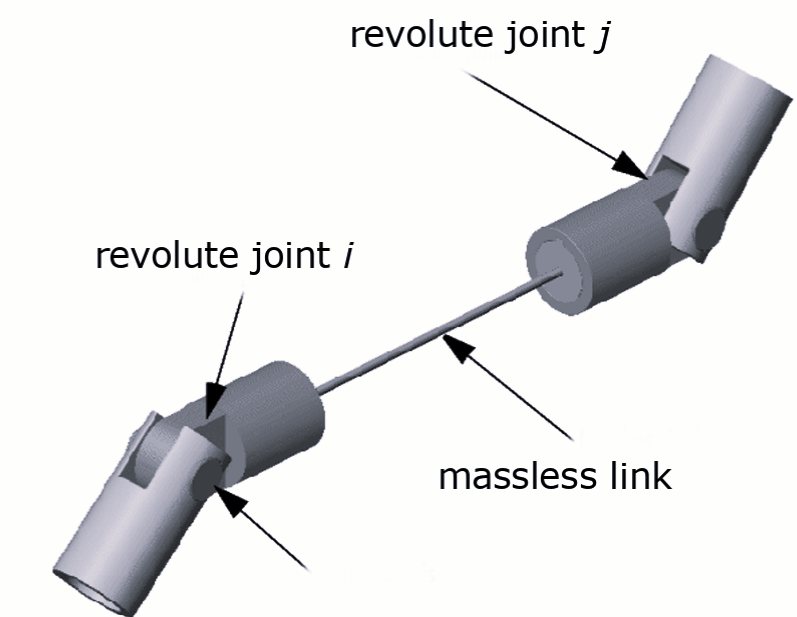
\includegraphics[scale=0.5]{img/joints_links.png}
    \caption{The robot joints are moved by actuators (eg. motors) and are connected by links/arm which are assumed to be massless}.
\end{figure}

\subsection{Types of joints}
In the following we will consider two types of joints: 
\begin{enumerate}
    \itemsep-0.3em
    \item \textsf{Revolute (or Rotational) joints} which allows a \textbf{rotation} between the connected links; 
    \item \textsf{Prismatic (or Traslational) joints} which allows a \textbf{translation} between the connected links.
\end{enumerate}

\begin{figure}
    \centering
    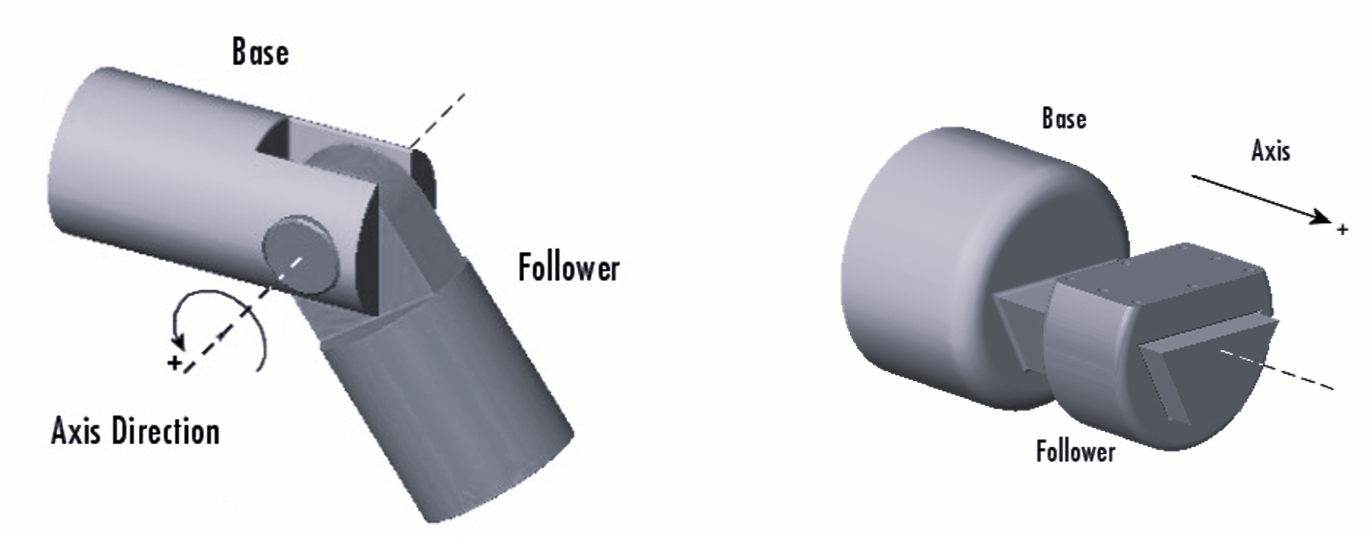
\includegraphics[scale=0.5]{img/joints_tyeps.png}
    \caption{Revolute and Prismatic joints. With a dashed line the direction of motion (axis) is indicated}
\end{figure}
According to the number of links we can find between any two joints, kinematic chains can be \textbf{open chains} or \textbf{closed chains}. In the former case there is only one link between any two links in a way joints and arms form a \textit{tree-like} structure; in the latter case there might be more than one link between any two joints, and in this case joints and arms are arranged in a \textit{cycle-like} structure.

\subsection{Graphical representation}
There are different types of graphical representations for kinematic chains, in the following we will use cylinders and boxes for joints, segment for links/arms. 

\begin{figure}
    \centering
    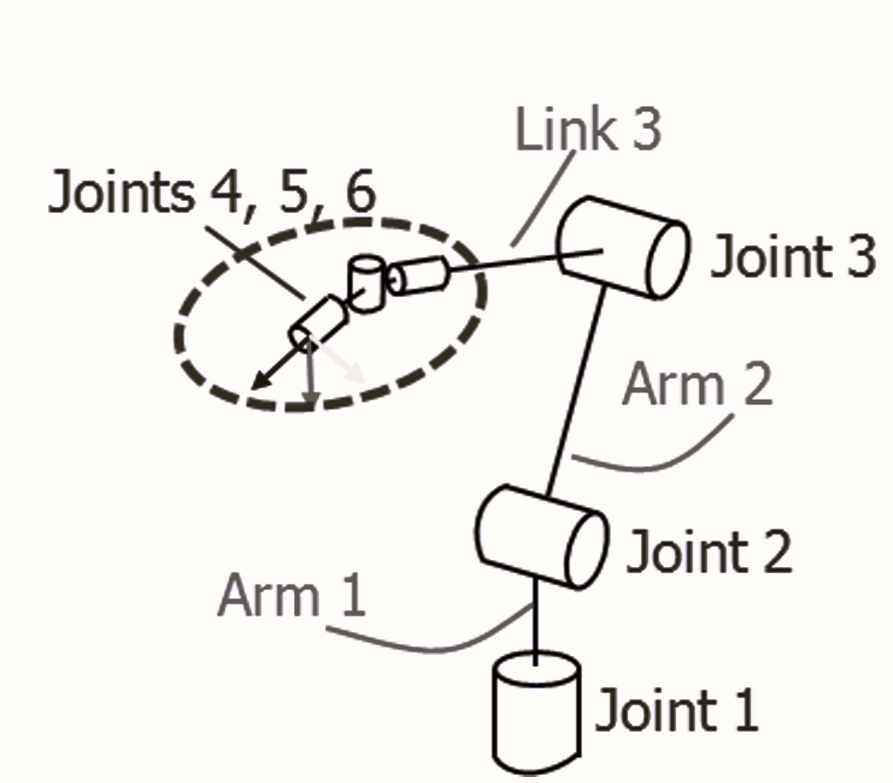
\includegraphics[scale=0.5]{img/KC_sample.png}
    \caption{Kinematic chain sample}
    \label{fig:KC_sample}
\end{figure}
More specifically \textit{\textbf{rotation joints}} are drawn in 3D has small cylinders withb the axes aligned along each rotation axis, in 2D they are drawn as small circles or small hourglasses.

\begin{figure}[h]
    \centering
    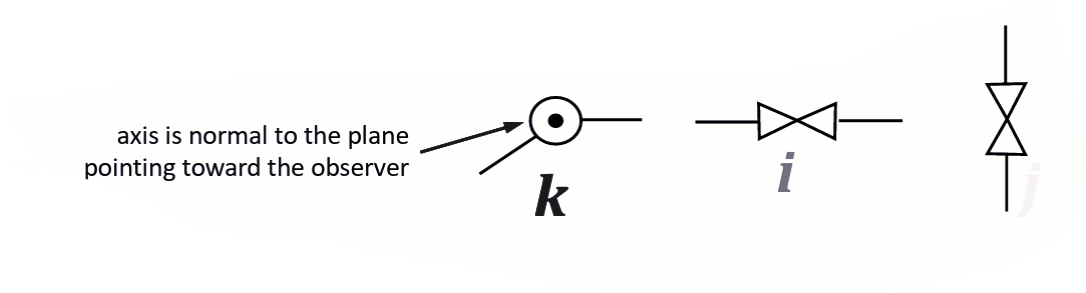
\includegraphics[scale=0.6]{img/rot_joints.png}
    \caption{2D-representation for revolute joints}
\end{figure}

At the opposite, \textit{\textbf{prismatic joints}} are represented as small boex with each axis aligned along the translation axis. On the other hand in 2D they are drawn as small squares with a point in their center, or as small rectangles showing the direction for the outcoming links.

\begin{figure}
    \centering
    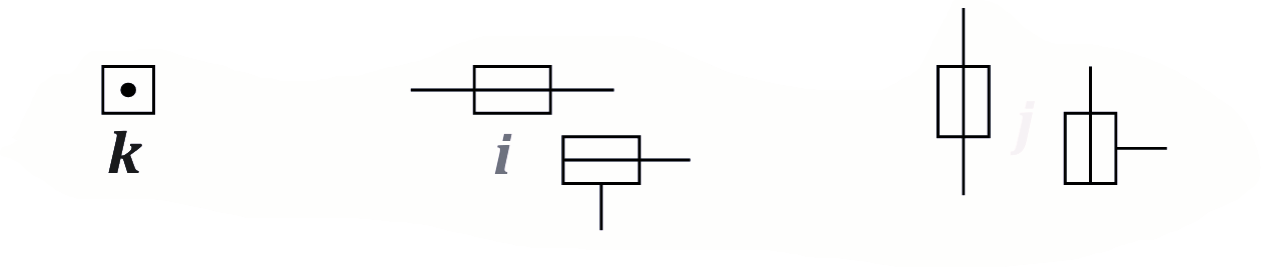
\includegraphics[scale=0.5]{img/transl_joints.png}
    \caption{2D representation of translational joints}
\end{figure}

\begin{figure}
    \centering
    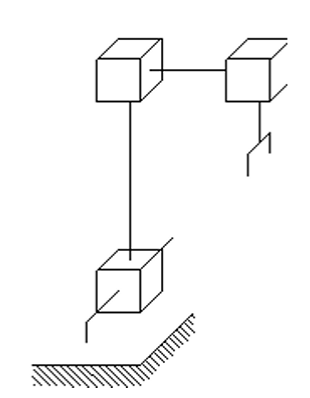
\includegraphics[scale=0.6]{img/transl_joints_3D.png}
    \caption{3D graphical representation for prismatic joints}
\end{figure}

\subsection{End-effector}
The \textbf{end-effector} (also called \textit{hand, gripper} or \textit{hand tool}) is the structure which is attached to the last link, and it is the one by which the task, for which that robot was introduced, can be executed. For the end effector a particular type of point is interesting, this is the \textbf{Tool Center Point (TCP)} and it is the baricenter of the hand, or better that ideal point that the robot software moves through the space. How we will see it is useful to attach to such a point a reference frame. \\
The graphical representation is used for the end-effector is a sort of fork. The end-effector can be of any type and we can draw and study the kineamtic chain without assuming the use of any particular hand.

\begin{figure}
    \centering
    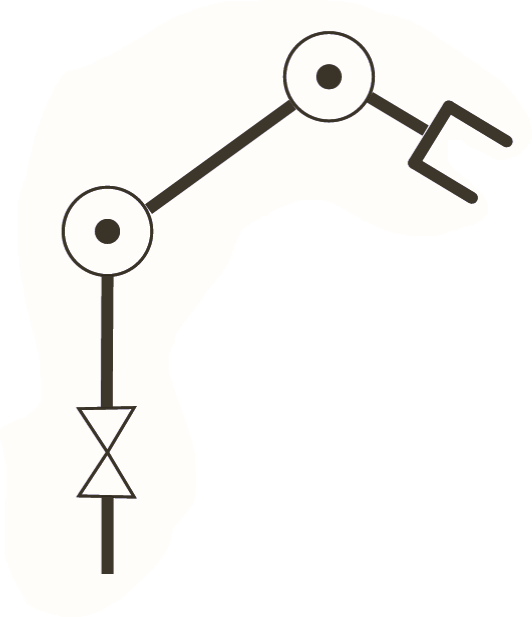
\includegraphics[scale=0.4]{img/endeff_graphical.png}
    \caption{End-effector graphical representation. Typically the TCP is assumed to be the center of the 'fork'}
\end{figure}




\section{Robot types}
An \textbf{Industrial manipulator} is usually composed by a \textbf{shoulder} and a \textbf{wrist}. The manipulators can be categorized according to the structure of their arms, which are based on the type of joints. We will indicate:
\begin{center}
    \underline{\textbf{R=revolute joint}}\\
    \underline{\textbf{P=Prismatic joint}}
\end{center}
A great number of robots can be obtain according the shoulder configuration, however in the industrial fields, few configurations are used which are more suitable for certain tasks instead of others. In the following we are going to explore the most common structures giving their main characteristics.

\subsection{Cartesian manipulator \texttt{(PPP)}}
\begin{multicols}{2}
    \begin{figure}[H]
        \centering
        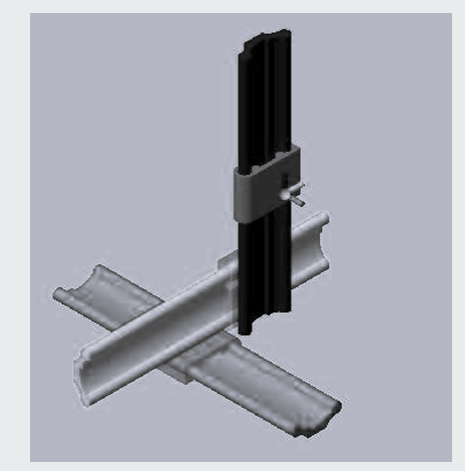
\includegraphics[scale=0.5]{img/man_cart.png}
        \caption{Cartesian manipulator structure}        
    \end{figure}
    \noindent
    In a \textbf{cartesian manipulator} the structure \texttt{(PPP)} is related to the shoulder structure. In this case the shoulder is composed of three prismatic joints, whose axis are mutually orthogonal. In this  case each degree of motion corrensponds to a cartesian variable. We anticipate that the task space is a sort of \textit{parallelepiped}. The figure aside shows an example of cartesian manipulator (taken from a robot simulator). Such robots have a good accuracy, while reguarding the dexterity cannot be said the same.
\end{multicols}
%------------------------------------------------------------
\subsection{Cylindrical manipulator \texttt{(RPP)}}
\begin{multicols}{2}
    \begin{figure}[H]
        \centering
        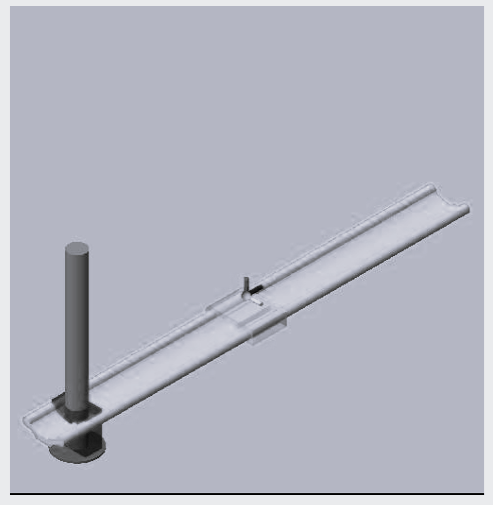
\includegraphics[scale=0.5]{img/cyl_man.png}
        \caption{Cylindrical manipulator structure}
    \end{figure}
    One rotoidal joint and two prismatic joints are the basic building blocks for the shoulder of a cylindrical manipulator. Here it is remarkable that for each DOM (from now on, degree of  motion) we have a cylindrical coordinate. The \textit{task space} is a \textbf{cylindrical sector}. The horizontal prismatic joint allows  to reach horizontal spaces, however here the accuracy decreases toward the arm ends.
\end{multicols}
\newpage
%------------------------------------------------------------

\subsection{Polar (or Spherical) manipulator \texttt{(RRP)}}
\begin{multicols}{2}
    \begin{figure}[H]
        \centering
        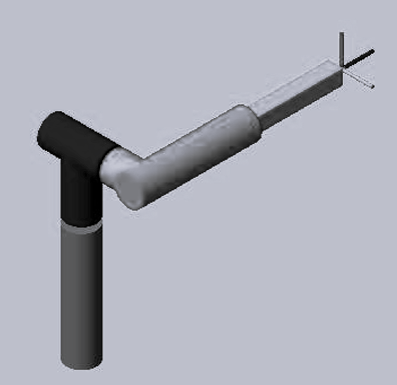
\includegraphics[scale=0.5]{img/spherical_man.png}
        \caption{Spherical manipulator structure}
    \end{figure}
    \noindent
    For a \textbf{polar (or spherical) manipulator} the shoulder has two revolute joints followed by a prismatic one. Each DOM corresponds to a polar coordinate; here the task is a spherical sector  that may include parts of the floor to allow manipulation of objects there located. The structure is less rigid wrt previous one, the accuracy reduces  with the elongation of the  prismatic arm.
\end{multicols}
%------------------------------------------------------------

\subsection{SCARA \texttt{(RRP)}}
\begin{multicols}{2}
    \begin{figure}[H]
        \centering
        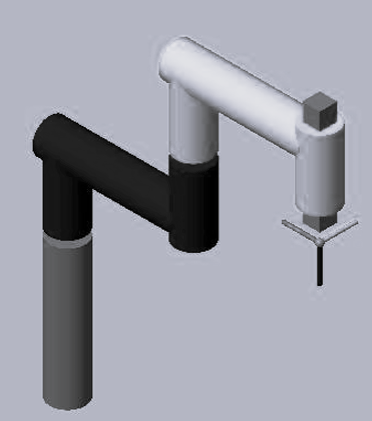
\includegraphics[scale=0.5]{img/scara.png}
        \caption{SCARA industrial robot structure}
    \end{figure}
    \noindent
    It is a robot used for \textit{pick and place} applications. The shoulder has two revolute joints followed by one prismatic joint, all with \textbf{parallel vertical axes}. The tasks addressed by this robot are the manipulation of small components or little assembly tasks.
\end{multicols}
%------------------------------------------------------------

\subsection{Antropomorphic (or articulated) manipultator \texttt{(RRR)}}
\begin{multicols}{2}
    \begin{figure}[H]
        \centering
        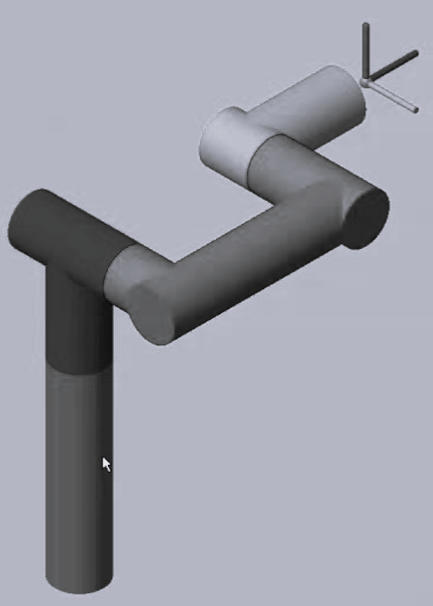
\includegraphics[scale=0.5]{img/antrop_man.png}
        \caption{Antropomorphic manipulator structure}
    \end{figure}
    The shoulder is composed of \textbf{three revolut joints}: the first one is vertical, the others are \textbf{horizontal and parallels}. It is one of the most common structure in industry, since it is the robot having \textbf{the best dexterity}.
\end{multicols}
%------------------------------------------------------------

\newpage
\subsection{Parallel robots}
\begin{multicols}{2}
    \begin{figure}[H]
        \centering
        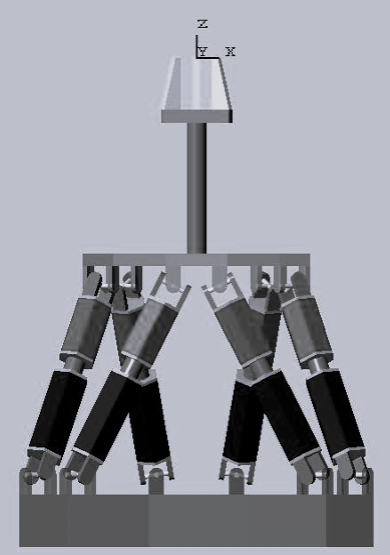
\includegraphics[scale=0.5]{img/parallel_man.png}
        \caption{Parallel manipulator (closed chain)}
    \end{figure}
    \noindent
    Such a type of manipulators have joints and links forming a cycle-like structure. They are not covered in these notes. An example is showed in the figure aside.
\end{multicols}

\section{Wrists}
The main scope of the \textbf{wrist} is to \textit{give an orientation} to the TCP. In fact, it can be said that the shoulder sets the \textbf{origin position}, while the \textbf{wrist} orients the TCP. \textit{Spherical wrists} are the most common. A wrist is said to be \textbf{spherical} if the three axes always intersect in a single point.Even if not spherical, due to its orientation function, the wrist is made up of \textbf{three rotational joints}.

\begin{figure}[h]
    \centering
    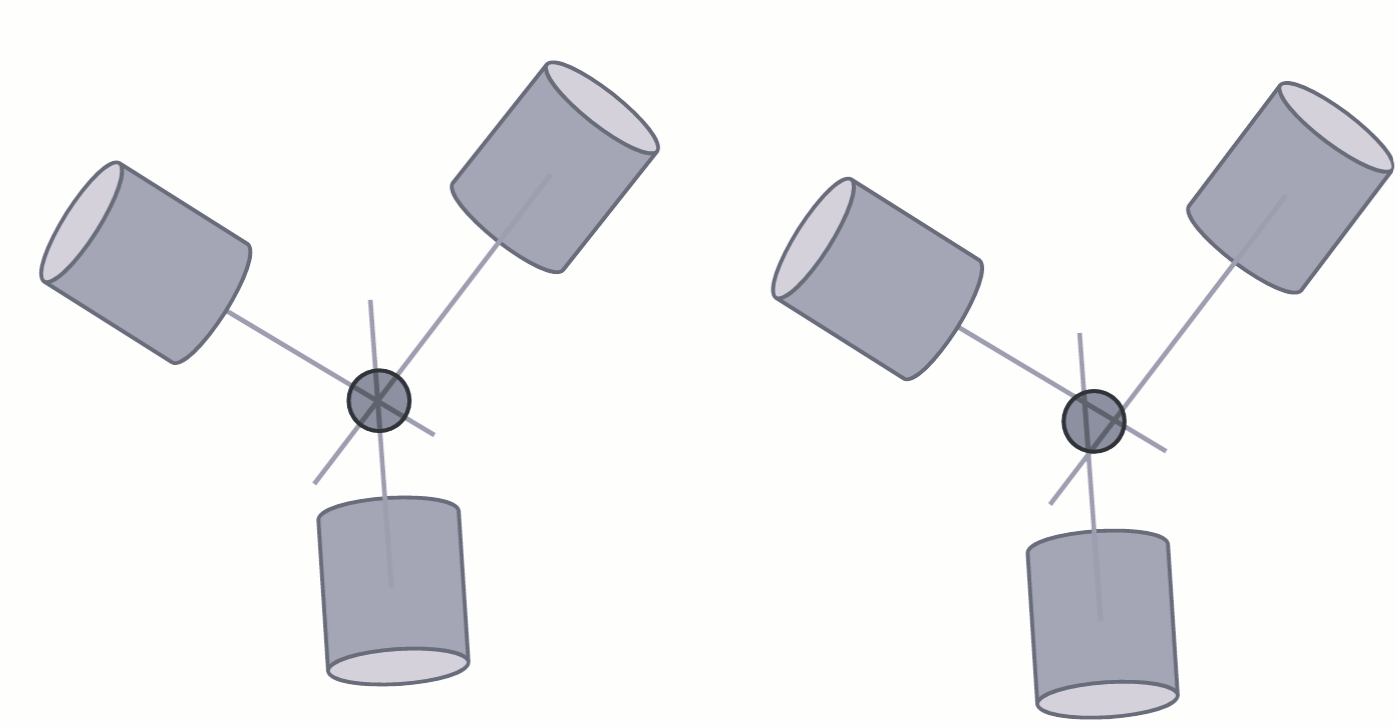
\includegraphics[scale=0.4]{img/sph_not_spherical.png}
    \caption{Spherical wrist (left) and Non-spherical wrist (right)}
\end{figure}
Taking into account a spherical joint, simplifies a lot the tractation of related topics of both manipulator kinematics and dynamics.
 
\section{Direct Kinematics}
\subsection{The Denavit-Hartemberg convention}
